\section{实验}
\label{sec:experiment}

\begin{figure*}[!ht]
 \centering
  \begin{minipage}[b]{\linewidth} 	
  \subfloat[]{
    \begin{minipage}[b]{0.5\linewidth} 
      \centering
      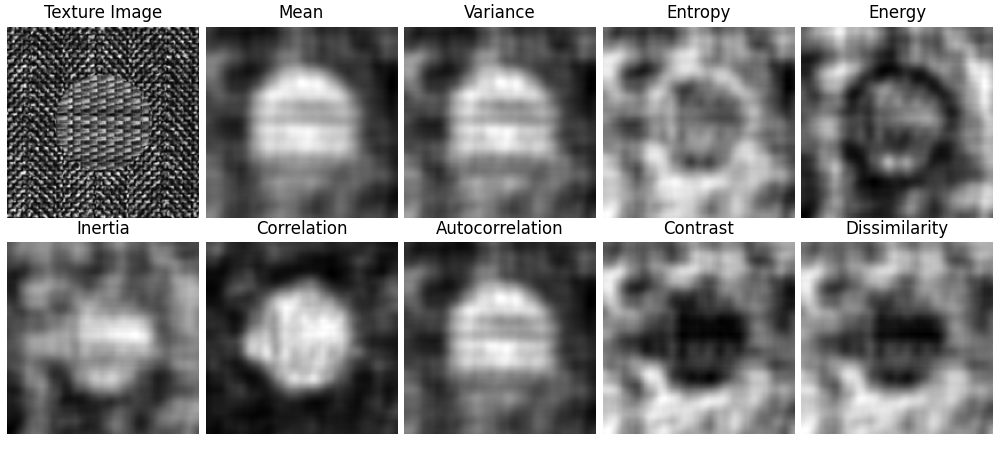
\includegraphics[width=\linewidth]{glcm_feats1}
       \end{minipage}
  }
%  \newline
    \subfloat[]{
    \begin{minipage}[b]{0.5\linewidth}
      \centering
      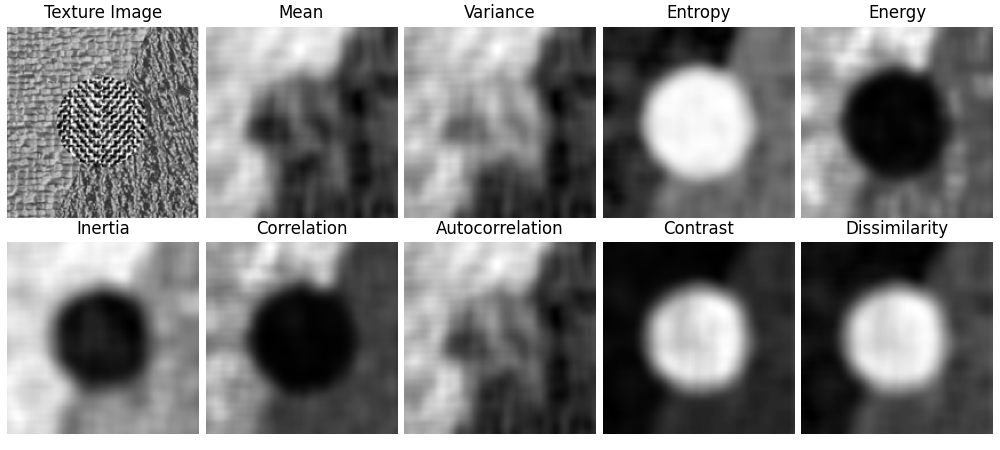
\includegraphics[width=\linewidth]{glcm_feats2}
     \end{minipage}
  }
  \newline
   \subfloat[]{
    \begin{minipage}[b]{0.5\linewidth}
      \centering
       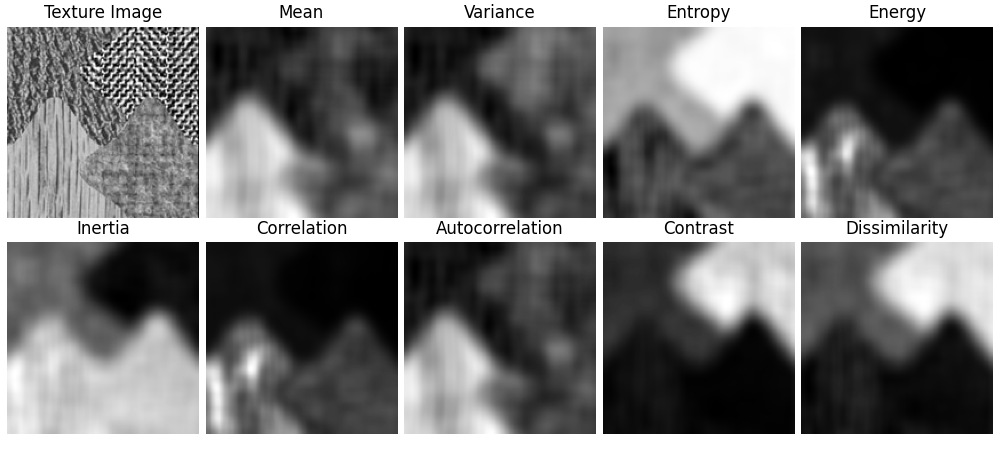
\includegraphics[width=\linewidth]{glcm_feats3}
       \end{minipage}
  }
    \subfloat[]{
    \begin{minipage}[b]{0.5\linewidth}
      \centering
      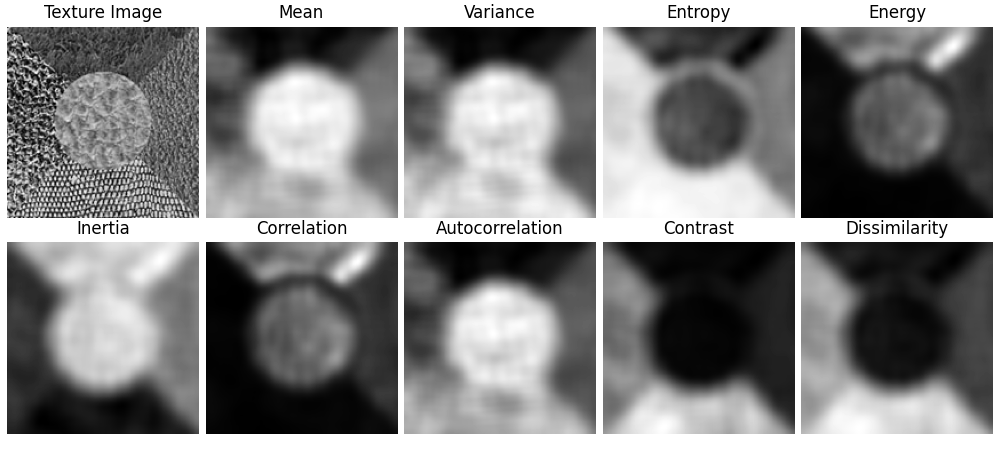
\includegraphics[width=\linewidth]{glcm_feats4}
     \end{minipage}
  }
  \end{minipage}
  \vfill
  \caption{灰度共生矩阵的统计特征可视化结果:(a) Texture\_mosaic\_1, (b) Texture\_mosaic\_2, (c)Texture\_mosaic\_3, (d) Texture\_mosaic\_4;第一行:纹理图像、Mean、Variance、Entropy、Energy;第二行:Inertia、Correlation、Autocorrelation、Contrast、Dissimilarity.}
  \label{fig:glcm_feats}
	
\end{figure*}

\begin{table*}[!htbp]
\caption{基于灰度共生矩阵的统计量及不同合成纹理图像指标选取示意表}
\centering
\label{tab:measurement}
\setlength{\tabcolsep}{3.5mm}{
\begin{tabular}{c|ccccccccc}
\hline
& Mean & Variance & Entropy & Energy & Inertia & Correlation & Autocorrelation & Contrast & Dissimilarity\\
\hline
1 & \checkmark & \checkmark & \checkmark & \checkmark & & \checkmark & & \checkmark &\\
2 & \checkmark & \checkmark & \checkmark & \checkmark & \checkmark & \checkmark & & &\\
3 & & \checkmark & \checkmark &  & \checkmark & & \checkmark & \checkmark & \checkmark\\
4 & \checkmark & \checkmark &  &  & \checkmark & & \checkmark & \checkmark & \checkmark\\
\hline
\end{tabular}}
\end{table*}

\subsection{灰度共生矩阵法的纹理分割实验}

如前文所述,在采用灰度共生矩阵法对纹理图像进行分割时,拟在表 \ref{tab:measurement} 中列出的统计量中进行选择用以对纹理进行表示和度量。因此本文首先先对测试图像的统计量结果进行了可视化处理,如图 \ref{fig:glcm_feats} 所示。在此基础上,根据不同统计量的可视化结果分别对测试图像使用的统计量进行选择,选取结果如表 \ref{tab:measurement} 所示。

在固定窗口大小为19,滑动步长为1,灰度等级为16的前提下,按照选取的统计量逐步计算各图像的灰度共生矩阵及相关统计量,并采用 K-Means 聚类方法对纹理图像进行分割,分割结果如图 \ref{fig:seg} 所示。

\begin{figure*}[!ht]
 \centering
  \begin{minipage}[b]{\linewidth} 	
  \subfloat[]{
    \begin{minipage}[b]{0.25\linewidth} 
      \centering
      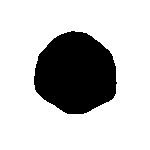
\includegraphics[width=\linewidth]{Texture_mosaic_1}
       \end{minipage}
  }
    \subfloat[]{
    \begin{minipage}[b]{0.25\linewidth}
      \centering
      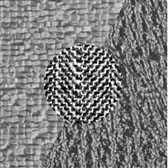
\includegraphics[width=\linewidth]{Texture_mosaic_2}
     \end{minipage}
  }
   \subfloat[]{
    \begin{minipage}[b]{0.25\linewidth}
      \centering
       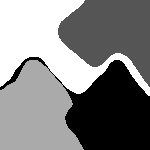
\includegraphics[width=\linewidth]{Texture_mosaic_3}
       \end{minipage}
  }
    \subfloat[]{
    \begin{minipage}[b]{0.25\linewidth}
      \centering
      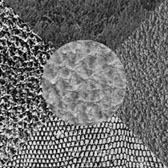
\includegraphics[width=\linewidth]{Texture_mosaic_4}
     \end{minipage}
  }
  \end{minipage}
  \vfill
  \caption{灰度共生矩阵的纹理分割结果:(a) Texture\_mosaic\_1, (b) Texture\_mosaic\_2, (c)Texture\_mosaic\_3, (d) Texture\_mosaic\_4.}
  \label{fig:seg}
	
\end{figure*}

分割结果受到窗口大小、滑动步长及聚类初始中心点的选择等因素的影响,文本将会在对比实验部分选择其中的一些因素对分割结果的影响进行探讨。

\subsection{Gabor 滤波器的纹理分割实验}

固定参数 Gabor 滤波器核的大小为 19,高斯窗口大小为 31,高斯函数的纵横比为 0.5,高斯窗口函数的标准差为 7,用于聚类的行和列的空间权重为 2,在这一参数条件下,Gabor 滤波器的纹理分割结果如图 \ref{fig:seg2} 所示。


\begin{figure*}[!ht]
 \centering
  \begin{minipage}[b]{\linewidth} 	
  \subfloat[]{
    \begin{minipage}[b]{0.25\linewidth} 
      \centering
      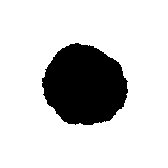
\includegraphics[width=\linewidth]{Texture_mosaic_1_gabor}
       \end{minipage}
  }
    \subfloat[]{
    \begin{minipage}[b]{0.25\linewidth}
      \centering
      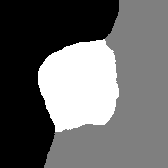
\includegraphics[width=\linewidth]{Texture_mosaic_2_gabor}
     \end{minipage}
  }
   \subfloat[]{
    \begin{minipage}[b]{0.25\linewidth}
      \centering
       
\includegraphics[width=\linewidth]{Texture_mosaic_3_gabor}
       \end{minipage}
  }
    \subfloat[]{
    \begin{minipage}[b]{0.25\linewidth}
      \centering
      
\includegraphics[width=\linewidth]{Texture_mosaic_4_gabor}
     \end{minipage}
  }
  \end{minipage}
  \vfill
%  \vspace{5mm}
  \caption{Gabor 滤波器的纹理分割结果:(a) Texture\_mosaic\_1, (b) Texture\_mosaic\_2, (c)Texture\_mosaic\_3, (d) Texture\_mosaic\_4.}
  \label{fig:seg2}	
\end{figure*}

  对比图 \ref{fig:seg} 来看,与灰度共生矩阵的纹理分割结果相比,如果忽略聚类初始中心点选择的影响,Gabor 滤波器的纹理分割结果在不同纹理的交界处的分割效果更好,这是由于其提取目标的局部空间和频率域信息方面具有良好的特性,且 Gabor 小波对于图像的边缘敏感,能够提供良好的方向选择和尺度选择特性,对噪声更加鲁棒。

\subsection{对比实验}

这一章节将在测试图片 Texture\_mosaic\_3 上对不同的参数进行调整,进行对比实验。为消除聚类初始中心点选择对分割结果的影响,根据图像特性,选择图像的四个四分位点作为聚类的初始中心。下面分别对滑动窗口大小和步长对分割结果的影响进行讨论分析。

\subsubsection{滑动窗口大小的影响}

在探究滑动窗口大小对纹理分割结果的影响时,固定其他参数不变,窗口大小分别选取 13、19、30和50,分割结果如图 \ref{fig:winsize_result} 所示。


\begin{figure}[!ht]
	\vspace{-0.8cm}
  \centering
  \begin{minipage}[b]{\linewidth} 	
  \subfloat[]{
    \begin{minipage}[b]{0.25\linewidth} 
      \centering
      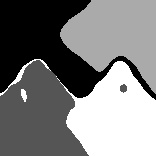
\includegraphics[width=\linewidth]{win_size_13}
       \end{minipage}
  }
    \subfloat[]{
    \begin{minipage}[b]{0.25\linewidth}
      \centering
      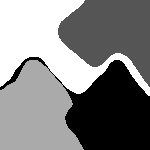
\includegraphics[width=\linewidth]{Texture_mosaic_3}
     \end{minipage}
  }
   \subfloat[]{
    \begin{minipage}[b]{0.25\linewidth}
      \centering
      
\includegraphics[width=\linewidth]{win_size_30}
       \end{minipage}
  }
	\subfloat[]{
    \begin{minipage}[b]{0.25\linewidth}
      \centering
      
\includegraphics[width=\linewidth]{win_size_50}
       \end{minipage}
  }

  \end{minipage}
  \vfill
  \caption{不同大小滑动窗口得到纹理分割结果:(a) $win\_size=13$, (b) $win\_size=19$, (c) $win\_size=30$, (d) $win\_size=50$.}
  \label{fig:winsize_result}
\end{figure}

从图 \ref{fig:winsize_result} 可以看出,当滑动窗口的选择偏小时,在区域内部会有被错分的较小区域,其原因可能是窗口的选择过小,导致对纹理特征的估计发生了错误。而随着窗口的增大,区域内部被错分的情况消失,但随之出现的是区域的交界处易被划分错误,其原因可能是窗口的选择过大,不能很好地捕捉到纹理的局部特性。

\subsubsection{滑动步长大小的影响}

在探究滑动步长大小对纹理分割结果的影响时,固定其他参数不变,步长大小分别选取 1、2和3,分割结果如图 \ref{fig:stride_result} 所示。

\begin{figure}[!ht]
	\vspace{-0.8cm}
  \centering
  \begin{minipage}[b]{\linewidth} 	
  \subfloat[]{
    \begin{minipage}[b]{0.3\linewidth} 
      \centering
      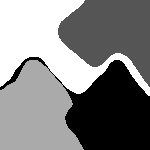
\includegraphics[width=\linewidth]{Texture_mosaic_3}
       \end{minipage}
  }
    \subfloat[]{
    \begin{minipage}[b]{0.3\linewidth}
      \centering
      
\includegraphics[width=\linewidth]{stride_2}
     \end{minipage}
  }
   \subfloat[]{
    \begin{minipage}[b]{0.3\linewidth}
      \centering
      
\includegraphics[width=\linewidth]{stride_3}
       \end{minipage}
  }
  \end{minipage}
  \vfill
  \caption{不同大小滑动步长得到纹理分割结果:(a) $stride=1$, (b) $stride=2$, (c) $stride=3$.}
  \label{fig:stride_result}
\end{figure}

从图 \ref{fig:stride_result} 可以看出,随着滑动步长的逐渐增大,分割边界逐渐变得不再平滑,呈现出锯齿状。

